\documentclass[a4paper,11pt,uplatex]{jsbook}
%\usepackage{fancyhdr}
\setlength{\footskip}{16pt}
\usepackage{amsmath}
\usepackage[dvipdfmx]{graphicx}
\usepackage[dvipdfmx]{color}
%\usepackage{pagecolor}[white]
\usepackage{amsmath,amssymb}
%\usepackage[top=3cm, bottom=3cm, left=3cm, right=3cm]{geometry}
\usepackage{braket}
\usepackage{bm}
\numberwithin{equation}{section}
\usepackage{mathrsfs}
\usepackage{siunitx}
\usepackage{physics}
\usepackage[dvipdfmx]{graphicx}
\usepackage[compat=1.1.0]{tikz-feynhand}
\usepackage{caption}
\usepackage{subcaption}
%\usepackage{cleveref}
\usepackage{float}
\usepackage{multicol}
\setlength{\columnsep}{15mm}
%\usepackage[style=phys,articletitle=false,biblabel=brackets,chaptertitle=false,pageranges=false]{biblatex}
%\usepackage[style=phys]{biblatex}
\usepackage[dvipdfmx]{hyperref}
\usepackage{url}
\usepackage{pxjahyper}
\usepackage{bookmark}
%\usepackage[backref]{hyperref}
\setcounter{tocdepth}{3}
\setlength{\parindent}{2em}
\def\vector#1{\mbox{\boldmath $#1$}}
\def\slash#1{\not\!#1}
\def\slashb#1{\not\!\!#1}
\def\delsla{\not\!\partial}
%\usepackage[dvipdfmx]{xcolor}


\hypersetup{
 setpagesize=false,
 bookmarksnumbered=true,%
 bookmarksopen=true,%
 colorlinks=true,%
 linkcolor=black,
 citecolor=red,
 urlcolor=black,
}
%backreferenceのカスタマイズ. "Back to p.3"のように表示する.
%\renewcommand*{\backref}[1]{(p.#1へ戻る)}
%\newcommand{\backtoc}{\hyperlink{toc}{[目次へ]}}
\newcommand{\backtoc}{\texorpdfstring{\protect\hyperlink{toc}{\hspace{5pt} \scriptsize [目次へ]}}{}}
\newcommand{\mychapter}[1]{\chapter[#1]{#1\backtoc}}
\newcommand{\mysection}[1]{\section[#1]{#1\backtoc}}
\newcommand{\mysubsection}[1]{\subsection[#1]{#1\backtoc}}

% 数式
%\usepackage{amsmath,amsfonts}
%\usepackage{bm}
%\usepackage{physics}
% 画像
%\usepackage[dvipdfmx]{graphicx}
%\usepackage[dvipdfmx,colorlinks=true,linkcolor=blue]{hyperref}
%\usepackage{pxjahyper}

\begin{document}


\chapter{MAMIにおける測定手法}
この章の目的は、実験に用いた装置の性能や仕様、およびセットアップの手法を説明することである。
また、データ取得の手順を示す。
\section{装置とセットアップ}
\subsection{マインツマイクロトロン(MAMI)}
Mainz Microtron(MAMI)はドイツ、マインツ大学が所有する連続電子線加速器施設である。最大エネルギー1508 MeVの電子ビームを供給する
3台のRTM(Race Track Microtron)および1台のHDSM(Harmonic Double Sided Micrtron)から構成される。
MAMIのフロアマップを図に、主なパラメータを表\ref{MAMI}に示した。
ハイパー核生成実験ではHDSMを用いて最大エネルギーの1508 MeVの電子ビームを供給する。

スペクトロメータ較正実験では、RTM3までで加速された180 MeVから210 MeVまでの電子ビームを用いる。
\begin{table}
  \caption{MAMIの主要パラメータ}\label{MAMI}
  \centering
  \begin{tabular}{c||cc}
    \hline
     &RTM3 & HDSM \\
    \hline
    最大エネルギー & 855.1 MeV & 1508 MeV \\
    最大強度 & 100 $\mu$A & 100 $\mu$A \\
    周回数 & 90 & 43 \\
    偏光磁石の磁場 &1.28 T & 0.95 - 1.53 T\\
    周波数 & 2.45 GHz & 2.45 / 4.9 GHz \\
    エネルギー幅 & 13 keV & 110 keV \\
    水平方向エミッタンス & 13 $\pi$ $\mu$m mrad & 27 $\pi$ $\mu$m mrad \\
    垂直方向エミッタンス & 0.84 $\pi$ $\mu$m mrad & 1.2 $\pi$ $\mu$m mrad\\
    \hline
  \end{tabular}
\end{table}
ここでは本研究で用いる200 MeV領域の電子ビームに注目し、RTM3における加速機構を説明する。
図??にRTM3の模式図を示した。2つの180$^\circ$偏向電磁石の間には線形加速器(LINAC)が設置されている。
前段の加速器で180 MeVまで加速され入射された電子はLINACで加速されるごとにおよそ15 MeVエネルギーを得る。加速されると偏向電磁石での軌道半径が大きくなり、
一つ外側の周回軌道を通り再びLINACで加速を受ける。このようにして電子は周回軌道を繰り返し、最終的に最大で855 MeVまで加速されて実験ホールに供給される。
周回軌道の途中にはビーム取り出しのためのキッカーマグネットが設置されており、このキッカーマグネットをどの軌道に設置するかによって周回回数を調節し、供給するエネルギーを決定する。

RTM3の直後には供給するビームラインを選ぶための偏向電磁石が設置されており極性をレバーで変えることで、アンジュレータ放射光干渉法による電子ビームエネルギー測定を行うX1ホールと、電子弾性散乱によるスペクトロメータ較正を行うA1ホールにビームを供給するモードを切り替えることができる。

\subsubsection{X1ホール}
電子ビームエネルギー測定を行うX1ホールの構成を図??に示す。
ビーム調整を行うsteerer電磁石はRTM3に設置されており、水平方向、垂直方向のビーム位置を調整する。
またX1ビームラインには4つの四重極磁石が配置されている。アラインメントの基準となるほか、ビーム調整でも利用するが、測定を行う際には原則利用しない。
2つ目の四重極電磁石と3つ目の四重極電磁石の間にアンジュレータが設置されている。
また4つ目の四重極電磁石の後方にビームプロファイルモニタが設置されている。

またX1ホール内には光学系の較正用の水銀灯や青色レーザー、ビームライン内の可動式ミラーが設置されている。
水銀灯や青色レーザーによる較正を行う際にはミラーボックス内のミラーをビームライン中心に移動させることで水銀灯や青色レーザーを光学系に供給することができる。
\subsubsection{ビーム調整}
まずビームプロファイルモニタを用いてフェイントビームの位置を目測で調整する。この時の精度は数 mm 程度である。
続いて、ビーム強度を5 $\si{\mu}\text{A}$に上げつつ放射線レベルが基準値よりも低くなるように微調整を行う。
この時放射線レベルが安全基準よりも高くなることは、ビームがビームダンプまで輸送されるまでにビームパイプ中心から外れていることを示す。
最後にカメラを用いて放射光を見ながらビームの位置を調整する。スリットに対してビーム中心がずれている場合には回折パターンが上下非対称になる。
\subsection{アンジュレータ}
アンジュレータは自作のコイルを用いて設計された。各コイル対が独立に制御可能な電磁石となっている。1台のアンジュレータに計13個のコイルが等間隔かつ極性が交互に配置されている。
各コイルの間隔は?? mmであり、上下のギャップは??mmである。ギャップサイズは固定し、電磁石による磁場調整を行う。全長が?? mmである。
\subsubsection{磁場制御}
各コイルには電源ボックスから電流を供給する。電流値を調整することで正弦波状の磁場を発生させることができる。
マトリックス型のホールプローブを用いて磁場を測定し、
隣り合う電磁石の磁場が影響するため、適切な磁場を得るためには全ての電磁石の電流を同時に調整する必要がある。
そのため、測定と電流のチューニングを繰り返し行う。
アンジュレータ通過後の電子ビームの方向のずれを最小に抑えることが重要となる。

\subsubsection{位置制御と読み取り}
アンジュレータは可動式ステージに取り付けられており、モーターによって移動させる。
可動範囲はビームライン上の制約から最大 825 mm、間隔は通常の測定では 5 mmで指定する。
移動したアンジュレータの絶対値は、リニアエンコーダ(Heidenhain LC415)で 5 $\mu \text{m}$ の精度で読み出すことができる。
\subsubsection{アラインメント}
セオドライトを用いてアンジュレータと較正用水銀灯、スリットの位置を調整した。セオドライトの基準はX1 Hallの壁に設置されたマーカーと四重極電磁石の中心で、
四重極電磁石はマーカーを基準に精密に水平に設置されていることが保証されている。
\subsection{分光光学系}
分光光学系全体の構成を図??に示す。各素子間の長さは、素子の中心同士を結ぶ直線をものさしで測定した。
放射光の光軸が必ずしも素子の中心を通ることは保証されていないため、測定誤差と合わせて全ての値に1 mmの誤差を見積もった。
\subsubsection{スリット}
矩形スリットを用いる。
スリット幅は4 mm(vert) x 6 mm(hori)であり、調節ねじにより上下、および左右のブレードが連動して動き、スリット幅を調整可能である。
これを$x$軸、$y$軸方向の可動ステージに乗せることでスリット全体の位置を0.1 mm単位で調整可能にした。
\subsubsection{grating}
回折格子はThorlab製の??を用いた。格子定数は800/mmである。ピッチ・ヨー方向に調節可能な光学マウントによって固定され、さらに光学マウントが水平方向の回転ステージに設置されている。
これにより分光された放射光がカメラ方向に水平に反射される。

\subsubsection{波長分散レンズ}
水平方向にのみ光波を収束する樽型レンズを用いた。焦点距離は1 m である。このレンズもピッチ・ヨー方向および$y$軸方向の調節が可能な光学マウントによって固定される。
\begin{figure}[tb]
  \centering
  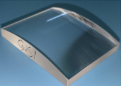
\includegraphics[width=0.8\linewidth]{image/3-lens.png}\\
  \caption{レンズ}
  \label{lens}
\end{figure}
水平墨出しレーザーの反射光を用いることでピッチ・ヨー回転の調整ができる。

\subsubsection{CMOS カメラ}
光学系は波長が400 nmの領域において働くため、可視光領域のカメラを用いることができる。HAMAMATSU C14440-20UPを用いた。
仕様を以下に示す。
\begin{table}[h]
\centering
\begin{tabular}{c|c}
  ピクセル数 & 2304 $\times$ 2304\\
  ピクセルサイズ & 6.5 $\mu$m $\times$ 6.5 $\mu$m\\
  チップサイズ & 14.976 mm $\times$ 14.976 mm\\
  ビット深さ & 16 bit\\ 
\end{tabular}
\end{table}

\subsection{光学系のアラインメント}
青色レーザを用いて光学系全体の光軸調整を行った。青色レーザーの光軸はセオドライトを用いてビームライン中心と合わせる。
ビーム中心と合わせた青色レーザー光を光学系に通し、各光学素子の中心をとおるようにアラインメントを行う。
またレーザー墨出し器を用いて光学系全体の水平を確認する。回折格子とレンズの水平は青色レーザー光の位置を基準に調整した。
\section{データ取得}


\subsection{分光光学系の波長較正}
波長較正として水銀灯を用いる。
$400 \text{nm}$領域には2本の輝線があり、このスペクトルを光学系で観測することで2つの輝線スペクトルを観測できる。\\
水銀灯ランプはビームラインから垂直に5 mの位置に設置されており、ミラーを用いて電子ビームラインと同じ軌道を通って光学系に導かれる。\\

輝線スペクトルをガウス関数でフィッティングし、中心位置のピクセルを対応する波長にする。
2本のスペクトル以外のピクセルは2本の輝線の波長 -ピクセル関係の線形性を仮定して決定する。
\subsection{データ取得}
\begin{itemize}
  \item 指定の位置にアンジュレータが移動する
  \item カメラによる画像撮影の信号が4回送られる
  \item 画像撮影が完了するとDAQに信号が送られる
  \item アンジュレータのモータに次の指定位置の信号が送られる
  \item アンジュレータが指定位置まで移動する。
\end{itemize}
\subsubsection{配線}

\subsection{電子ビームエネルギー測定}

ビームラインの切り替え\\
プロファイルモニタによるビームチューニング\\
画像によるビームチューニング\\

\subsection{弾性散乱実験との同時運用}
弾性散乱実験と並行してアンジュレータによる電子ビームエネルギー測定を行った。
基本的なランプランは、弾性散乱実験の前後にエネルギー測定を行う形である。
\subsection{下流側アンジュレータによるデータ測定}
パラメータ較正を目的として、下流側アンジュレータのみを用いたデータ取得を行う。


\end{document}